\section{Desarrollo del \textit{backend}}
\label{dev:sec:desarrollo_backend}

Una vez se ha definido la base de datos, uno ya puede tener una idea general de como puede funcionar la lógica de la aplicación. Al fin y al cabo, se debe entender el \textit{backend} como el elemento que permite a la aplicación gestionar los datos y aplicarles cierta lógica para que esta realice las operaciones que el usuario ordena desde el \textit{frontend}.

De este modo, como ya se ha comentado en la sección \ref{subsec:backend}, el \textit{backend} se ha desarrollado utilizando el \textit{framework} Django. Esta decisión es resultado de la experiencia previa con este \textit{framework}, de la experiencia en programación con Python y del hecho de que Django es uno de los \textit{frameworks} más utilizados para el desarrollo \textit{backend}. Cabe mencionar que además es un \textit{framework} categorizado como \textit{batteries included}, lo que significa que incluye muchas funcionalidades ya implementadas. Algunas de estas funcionalidades son la gestión de usuarios y seguridad, detallada en la sección \ref{subsubsec:usuarios_autenticacion}, y la gestión de la base de datos mediante un ORM, detallada en la sección \ref{mt:subsec:base_datos}. Hacer uso de estas funcionalidades es una bastante buena práctica en fases iniciales de desarrollo, ya que permite centrarse en la lógica de la aplicación y no en la implementación de funcionalidades que ya están disponibles, además de que estas funcionalidades considerablemente complejas, pero que son muy comunes en todas las aplicaciones. Adicionalmente, son funcionalidades seguras y que normalmente ofrecen buenos patrones de diseño, a pesar de que a no son tan flexibles y escalables como si se implementaran desde cero.

Por otro lado, Django tiene la opción de crear páginas mediante plantillas, lo que permite crear una aplicación web completa con un \textit{frontend} y un \textit{backend} en el mismo proyecto, es decir, sin salir de la propia infraestructura del \textit{framework}. Sin embargo, siguiendo lo comentado en la sección \ref{dev:subsec:separacion_frontend_backend}, está práctica es poco usada en la actualidad, ya que no permite crear aplicaciones dinámicas, pues por cada pequeño cambio de la página el servidor tiene que procesar la petición y devolver la página completa. Por poner un ejemplo, si se quiere mostrar una lista de elementos y se quiere añadir un nuevo elemento, el servidor tiene que procesar la petición, generar la página completa con la lista de elementos actualizada y devolverla al cliente, lo que supone una recarga de la página. Esto, a pesar de ser funcional y ser la norma algunos años atrás, ofrece una experiencia de usuario bastante pobre, lo que hoy en día no es aceptable. Por estos mismos motivos, se ha optado por crear un \textit{backend} que sirva una API RESTful, que es la norma en la actualidad, y un \textit{frontend} que consuma dicha API. Para ello, se ha utilizado Django REST Framework, una extensión de Django que permite crear APIs de tipo REST ofreciendo funcionalidades como la serialización de datos, la autenticación y la autorización, entre otras.

Con todo esto definido, para dejar descrito todo el \textit{backend} de la aplicación, se ha seguido un proceso de desarrollo que se detalla a continuación. Este proceso se ha dividido en varias secciones, cada una de las cuales se centra en un aspecto concreto del desarrollo del \textit{backend}. Así pues, se ha comenzado por la estructuración del proyecto, que es la base sobre la que se construirá el resto del \textit{backend}. A continuación, se han definido los modelos, que son la representación de los datos en la base de datos. Después, se han establecido los \textit{serializers}, que son los encargados de convertir los modelos en datos JSON y viceversa para así formalizar la API REST. Finalmente, se han desarrollado las vistas y las URLs, que son las encargadas de gestionar las peticiones y respuestas de la API.

\subsection{Estructuración del proyecto}
\label{dev:subsec:estructura_proyecto}

La estructuración del proyecto es un paso fundamental en el desarrollo de cualquier parte de la aplicación, ya sea el \textit{backend} como el \textit{frontend}. Estructurar correctamente permite organizar el código de manera que sea fácil de entender y mantener para que en un futuro se puedan añadir funcionalidades sin alterar la estructura ya existente. Cada \textit{framework} tiene su propio patrón de organización, el cual se recomienda para que el desarrollo sea lo más óptimo posible y en un futuro permita su escalabilidad.

Un proyecto de Django se compone de una serie de aplicaciones, cada una de las cuales se encarga de ofrecer una funcionalidad concreta. Dentro de cada aplicación, la estructura es la misma, de manera que cada aplicación tiene su propio directorio con los siguientes principales ficheros:

\begin{itemize}
    \item \texttt{models.py}: Es donde se definen los modelos de la aplicación.
    \item \texttt{serializers.py}: Es donde se definen los \textit{serializers} de la aplicación.
    \item \texttt{views.py}: Es donde se definen las vistas de la aplicación.
    \item \texttt{urls.py}: Es donde se definen las URLs de la aplicación.
    \item \texttt{admin.py}: Es donde se definen las configuraciones del panel de administración de Django.
\end{itemize}

Cada uno de estos ficheros van a ser detallados en las siguientes secciones, pues su importancia es fundamental para que el \textit{backend} funcione correctamente. En la figura \ref{dev:fig:estructura_django} se puede ver un ejemplo de la estructura de un proyecto de Django, donde se pueden observar las aplicaciones y los ficheros que componen cada una de ellas.

\begin{figure}
    \centering
    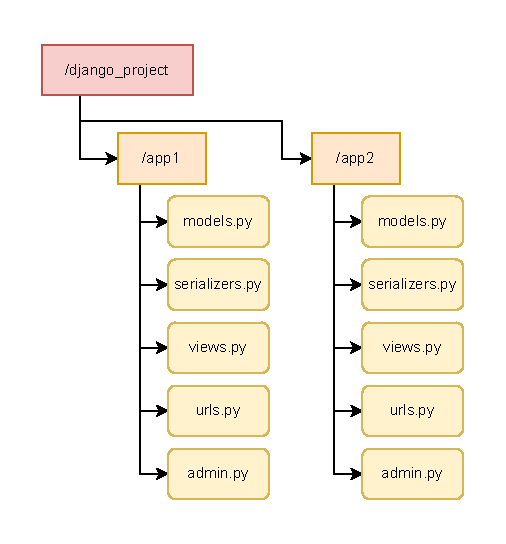
\includegraphics[width=0.6\textwidth]{figures/design_develop/estructura_django.pdf}
    \caption{Estructura de un proyecto de Django.}
    \label{dev:fig:estructura_django}
\end{figure}

En este proyecto, la decisión sobre cómo estructurar las funcionalidades no ha sido trivial. Si bien es cierto que se pueden identificar dos usos principales, la gestión de pedidos y la gestión de productos, ninguno de ellos es completamente independiente del otro. De hecho, ambos están estrechamente relacionados en distintos puntos del flujo de trabajo: los pedidos tienen productos asociados.

Además, la gestión de los \textit{marketplaces}, aunque actualmente no concentra una lógica compleja, constituye un pilar fundamental de la aplicación. No solo es un eje que articula tanto productos como pedidos, sino que también representa un área con un gran potencial de crecimiento. En el futuro, es probable que esta parte del proyecto incorpore nuevas funcionalidades relacionadas con integraciones, sincronización de datos o reglas específicas por canal de venta, lo que justifica su separación en una aplicación propia desde el inicio.

Precisamente por estas razones, se ha optado por separar la aplicación en tres módulos/aplicaciones independientes: orders, products y marketplaces. Esta división permite una mejor organización del código, una separación clara de responsabilidades y una mayor facilidad para escalar y mantener el proyecto a medida que crece. Aunque existen relaciones entre los distintos dominios, mantenerlos como apps independientes mejora la cohesión interna de cada uno y facilita enormemente que en un futuro se puedan añadir nuevas funcionalidades o modificar las existentes sin afectar al resto del sistema.

En conclusión, el proyecto quedará estructurado en un total de 3 aplicaciones, es decir, tres directorios, cada uno de los cuales contendrá los ficheros mencionados anteriormente. Dicha estructura se puede ver en la figura \ref{dev:fig:estructura_proyecto}.

\begin{figure}
    \centering
    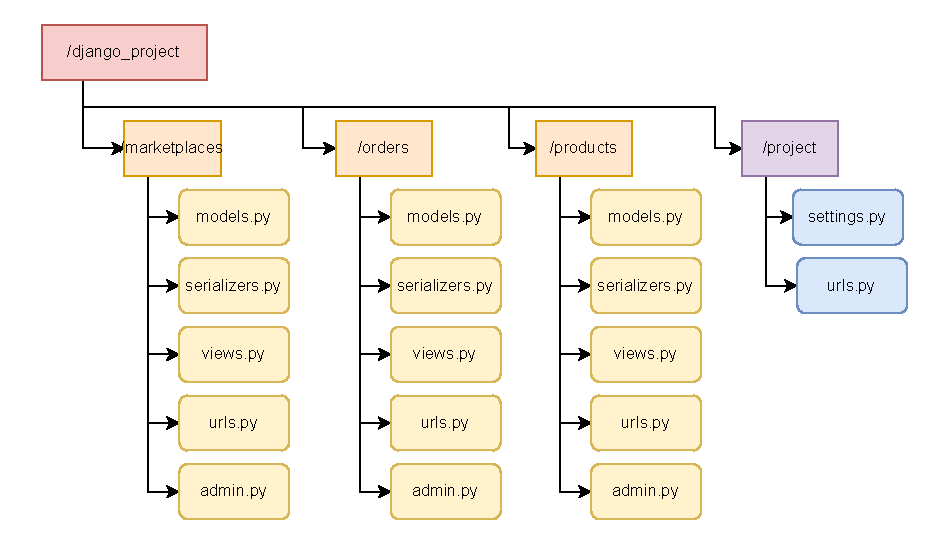
\includegraphics[width=0.8\textwidth]{figures/design_develop/estructura_proyecto.pdf}
    \caption{Estructura del proyecto.}
    \label{dev:fig:estructura_proyecto}
\end{figure}

Sin embargo, y ya para terminar, cabe mencionar un directorio adicional que se puede observar en la anterior figura \ref{dev:fig:estructura_proyecto}, el directorio project. Este directorio no es una aplicación, sino que es el directorio principal del proyecto. En este se encuentran los ficheros de configuración del proyecto, como el fichero \texttt{settings.py}, que contiene la configuración del proyecto como podría ser la configuración de la base de datos, y el fichero \texttt{urls.py}, que contiene las URLs del proyecto. Al primero no se la dará mucha relevancia en esta memoria, ya que, a pesar de ser muy importante, sale un poco del alcance. Sin embargo, el segundo sí que se va a detallar, ya que es donde se definen las URLs que apuntan a cada aplicación. En la sección \ref{dev:subsec:definicion_vistas_urls} se explicará cómo se definen dichas URLs y cómo se conectan con las vistas, que son las encargadas de gestionar las peticiones y respuestas de la API.

\subsection{Definición de los modelos}
\label{dev:subsec:definicion_modelos}

Con la estructura del proyecto definida, el siguiente paso es definir los modelos. Como se explicó en la sección \ref{mt:subsec:base_datos}, Django incluye de forma nativa un ORM que permite definir las tablas de la base de datos mediante clases de Python, y sus registros mediante objetos de esas clases. Con esto, se puede definir la base de datos y hacer consultas a la misma de una manera mucho más sencilla y rápida, ya que no es necesario escribir consultas SQL, sino que se pueden utilizar los métodos del ORM para realizar las operaciones necesarias.

Cada tabla de la base de datos es llamada modelo, y cada modelo se define mediante una clase de Python. Cada atributo de la clase representa una columna de la tabla, y cada instancia de la clase representa un registro de la tabla. Además, Django ofrece una serie de tipos de datos que se pueden utilizar para definir los atributos de las clases, como \texttt{CharField} para cadenas de texto, \texttt{IntegerField} para enteros, \texttt{DateTimeField} para fechas y horas, entre otros.

De esta manera, habiendo diseñado ya la estructura de la base de datos en la sección \ref{mt:subsec:base_datos}, definir los modelos es un proceso relativamente sencillo. Volviendo a la división en bloques de funcionalidades hecha en la sección \ref{dev:subsec:bloques_funcionalidades}, uno puede observar que, exceptuando el bloque de usuarios y autenticación, los tres bloques restantes corresponden a las tres aplicaciones que se han definido en la sección \ref{dev:subsec:estructura_proyecto}. Por lo tanto, las tablas de cada uno de los bloques se encontrarán definidas en el archivo \texttt{models.py} de cada una de las aplicaciones.

Dentro de cada uno de los ficheros \texttt{models.py} se definen las clases que representan los modelos de la aplicación. Cada clase hereda de \texttt{models.Model}, que es la clase base de Django para todos los modelos. A continuación, se definen los atributos de la clase, que son los campos de la tabla. Cada campo se define como un atributo de la clase y se le asigna un tipo de dato, como \texttt{CharField}, \texttt{IntegerField}, \texttt{DateTimeField}, entre otro. Además, se pueden definir relaciones entre modelos utilizando los campos \texttt{ForeignKey}, \texttt{ManyToManyField} y \texttt{OneToOneField}, dependiendo de la relación entre tablas que se quiera establecer.

\begin{center}
    \begin{minipage}{0.8\textwidth}
        \lstinputlisting[language=Python, caption={Definición del modelo \texttt{Product} para definir la tabla \texttt{product}.}, label={lst:model}]{listings/model.py}
    \end{minipage}
\end{center}

En el fragmento de código \ref{lst:model} se puede ver un ejemplo de cómo se ha definido el modelo \texttt{Product}. Cada uno de los atributos de la clase representa una columna de la tabla \texttt{product} de la base de datos, tal como pudo ser observado en la sección \ref{mt:subsec:base_datos}, y cada uno de los tipos de datos utilizados corresponde a un tipo de dato de la base de datos. Por ejemplo, el atributo \texttt{price} es un campo de tipo \texttt{DecimalField}, que corresponde a una columna de tipo \texttt{decimal} llamada \texttt{price} de la table \texttt{product} de la base de datos. Además, cada atributo tiene una serie de parámetros que permiten definir características adicionales del campo. Siguiendo el ejemplo, el atributo \texttt{price} tiene los parámetros \texttt{max\_digits} y \texttt{decimal\_places}, que permiten definir el número máximo de dígitos y el número de decimales que se pueden almacenar en el campo, respectivamente. Estos parámetros son muy útiles para garantizar la integridad de los datos y evitar errores al almacenar información en la base de datos.

Así pues, siguiendo cada uno de los bloques de funcionalidades definidos \ref{dev:subsec:bloques_funcionalidades} y la estructura entre aplicaciones establecida en la sección \ref{dev:subsec:estructura_proyecto}, se han definido los modelos siguiendo la figura \ref{dev:fig:estructura_modelos}. Como es observable, cada fichero \texttt{models.py} almacena los modelos del bloque de funcionalidades correspondiente a cada aplicación, de manera que en caso de que se quiera añadir un nuevo modelo, este se puede añadir en el fichero correspondiente sin alterar la estructura del proyecto.

\begin{figure}
    \centering
    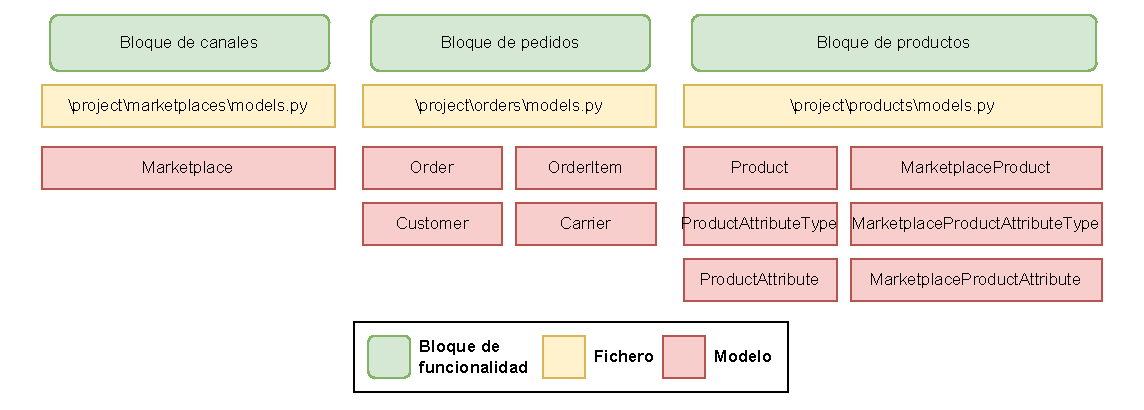
\includegraphics[width=0.8\textwidth]{figures/design_develop/estructura_modelos.pdf}
    \caption{Estructura de los modelos del proyecto.}
    \label{dev:fig:estructura_modelos}
\end{figure}

\subsection{Definición de los \textit{serializers}}
\label{dev:subsec:definicion_serializers}

Una vez definidos los modelos, el siguiente paso es crear los \textit{serializers}. Aunque en la práctica la definición de \textit{serializers} y vistas suele realizarse de forma conjunta, ya que las vistas necesitan los \textit{serializers} para enviar y recibir datos desde el \textit{frontend}, y estos carecen de utilidad sin una vista que los utilice, desde el punto de vista didáctico resulta más natural presentar primero la estructura de los \textit{serializers} y, a continuación, su uso dentro de las vistas. Por esta razón, en lugar de seguir el orden habitual, se explicarán primero los \textit{serializers} y después las vistas, en la correspondiente sección \ref{dev:subsec:definicion_vistas_urls}.

Con esta previa aclaración hecha, se puede empezar a definir que son los \textit{serializers} y cuál es su función dentro del \textit{backend}. Volviendo a la sección \ref{mt:subsec:api}, se ha comentado que la respuesta de una API REST acostumbra ser en un formato estructurado llamado JSON. Este formato es fácil de leer y entender, tanto para humanos como para máquinas, y es el estándar de facto para las APIs REST. Sin embargo, los datos que se manejan en el \textit{backend} suelen ser más complejos, ya que están representados por los modelos, que son objetos de Python. Por lo tanto, para poder enviar y recibir datos entre el \textit{frontend} y el \textit{backend}, es necesario convertir estos objetos en un formato más sencillo y manejable, como JSON. De esta manera, en términos generales, los \textit{serializers} son componentes que permiten convertir datos complejos, como los modelos, en formatos más simples y manejables. Un \textit{serializer} toma un modelo o un conjunto de datos y los convierte en formato JSON para que puedan ser enviados al \textit{frontend} y que este los pueda interpretar. De esta manera, tal como puede observarse en la figura \ref{dev:fig:serializer}, los \textit{serializers} eliminan el nivel de abstracción de los modelos convirtiéndolos en un formato que no deja de ser nada más que un conjunto de texto estructurado.

\begin{figure}
    \centering
    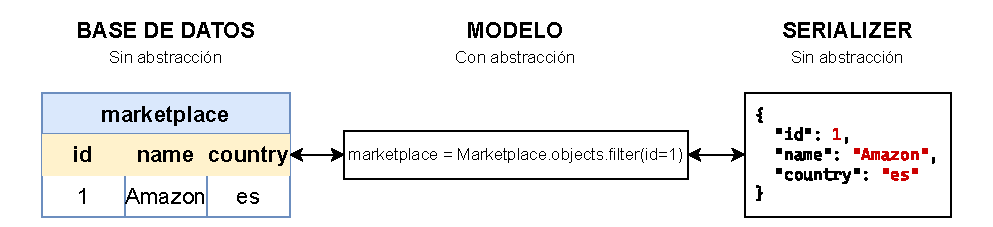
\includegraphics[width=0.8\textwidth]{figures/design_develop/serializers.pdf}
    \caption{Funcionamiento de los \textit{serializers}.}
    \label{dev:fig:serializer}
\end{figure}

No obstante, también tienen una función inversa, que es la de convertir datos en formato JSON en objetos de Python, lo que permite recibir datos desde el \textit{frontend} y transformarlos en objetos que se puedan manipular en el \textit{backend}. Todo esto, acompañado de una validación de los datos, ya que los \textit{serializers} también se encargan de validar que los datos recibidos cumplen con las reglas definidas en los modelos. Por ejemplo, si se recibe un dato que no es del tipo correcto o que no cumple con las restricciones definidas en el modelo, el \textit{serializer} devolverá un error indicando qué dato es incorrecto y por qué. Esto es muy útil para evitar errores en el \textit{backend} y garantizar que los datos que este trata son válidos y cumplen con las reglas definidas.

Con el concepto de \textit{serializer} ya definido, se puede empezar a ver como estos se estructuran dentro de Django. Como ya pudo ser observado en la figura \ref{dev:fig:estructura_proyecto}, cada aplicación tiene su propio fichero \texttt{serializers.py}, donde se definen los \textit{serializers} del bloque de funcionalidades correspondiente, de manera análoga a los modelos. Cada \textit{serializer} se define como una clase que hereda de \texttt{serializers.ModelSerializer}, que es la clase base de Django REST Framework para los \textit{serializers} basados en modelos. Al estar basada en modelos, esta clase permite definir los campos del \textit{serializer} de forma automática a partir de los modelos definidos en el fichero \texttt{models.py}. Esto significa que no es necesario definir manualmente cada campo del \textit{serializer}, sino que se pueden utilizar los campos del modelo directamente, lo que simplifica mucho su definición y, en caso de actualizar un modelo, no es necesario actualizar el \textit{serializer} manualmente, ya que este se actualizará automáticamente. Existe la posibilidad de hacer \textit{serializers} sin modelos, pero en este caso, donde el interés de la API es exponer los modelos de la base de datos, no tiene sentido hacer \textit{serializers} sin modelos. Adicionalmente, los \textit{serializers} basados en modelos también ofrecen la posibilidad de definir campos adicionales que no están presentes en el modelo, lo que permite añadir información extra al \textit{serializer} sin necesidad de modificar el modelo. Esto es muy útil para añadir información adicional que no es necesaria en la base de datos, pero que sí es útil para el \textit{frontend}. Por último, también existe la posibilidad de anidar \textit{serializers} dentro de otros, de manera que se pueden crear \textit{serializers} más complejos que representen relaciones entre modelos. Esto es muy útil para representar relaciones de tipo uno a muchos o muchos a muchos, ya que permite incluir información de los modelos relacionados dentro del mismo \textit{serializer}.

\begin{center}
    \begin{minipage}{0.8\textwidth}
        \lstinputlisting[language=Python, caption={Definición de los \textit{serializers} \texttt{Customer},  \texttt{OrderItem} y \texttt{Order}.}, label={lst:serializer}]{listings/serializer.py}
    \end{minipage}
\end{center}

En el fragmento de código \ref{lst:serializer} se puede ver un ejemplo de cómo se han definido los \textit{serializers} \texttt{Customer}, \texttt{OrderItem} y \texttt{Order}. Como se puede observar, el \textit{serializer} de \texttt{Order} incluye los \textit{serializers} de \texttt{Customer} y \texttt{OrderItem} como campos anidados, lo que permite incluir información de los modelos relacionados dentro del mismo \textit{serializer}. Con este se consigue que en el momento de serializar un pedido, los campos del cliente y los productos del pedido se incluyan dentro del mismo \textit{serializer}, lo que permite que con una sola petición se obtenga toda la información necesaria para mostrar un pedido completo. Dicha serialización se puede observar en el fragmento JSON \ref{lst:serializer_json}, donde se muestra el resultado del \textit{serializer} del modelo \texttt{Order} del fragmento \ref{lst:serializer}. Sin embargo, anidar campos no siempre es la mejor opción, pues muchas veces el \textit{frontend} no requiere de toda la información de los modelos relacionados, sino que solo necesita una parte y, como mayor sea la cantidad de información que se envíe, mayor será el tamaño de la respuesta y más lenta será la carga de la página. Por lo tanto, es importante tener en cuenta qué información es necesaria y cuál no, y anidar los campos solo cuando sea necesario.

\begin{center}
    \captionsetup{type=lstlisting, aboveskip=2mm, belowskip=2mm}
    \setlength{\fboxsep}{1pt}
    \begin{minipage}[t]{0.48\textwidth}
        \lstinputlisting[
            language=json,
            caption=
        ]{listings/order1.json}
    \end{minipage}
    \hfill
    \begin{minipage}[t]{0.48\textwidth}
        \lstinputlisting[
            language=json,
            caption=
        ]{listings/order2.json}
    \end{minipage}
    \vspace{2mm}
    \captionof{lstlisting}{Serialización de un pedido mediante el \textit{serializer} \texttt{Order} y los correspondientes \textit{serializers} \texttt{Customer} y \texttt{OrderItem} anidados.}
    \label{lst:serializer_json}
\end{center}

Precisamente por este último punto, la definición de los \textit{serializers} ha sido una de las tareas más complejas no solo del desarrollo del \textit{backend}, sino de toda la aplicación. A la hora de tomar decisiones sobre su estructura, se han tenido en cuenta tres aspectos clave:

\begin{enumerate}
    \item \textbf{Reutilización y generalización del código:} \\
          En el desarrollo de software, es habitual intentar que el código sea lo más genérico posible para favorecer su reutilización en diferentes partes de la aplicación. Esta práctica, aunque muy extendida, puede tener inconvenientes si se lleva al extremo, ya que un código excesivamente genérico puede resultar difícil de entender, mantener y, en algunos casos, poco eficiente.
    \item \textbf{Serializadores excesivamente completos:} \\
          Una posible estrategia consiste en crear un único \textit{serializer} que incluya todos los campos del modelo, además de anidar los \textit{serializers} de todos los modelos relacionados. Este enfoque puede ser útil en situaciones concretas, como al mostrar una vista detallada de un único pedido. No obstante, se vuelve ineficiente y poco adecuado si el objetivo es, por ejemplo, listar múltiples pedidos, ya que se estarían transmitiendo muchos datos innecesarios.
    \item \textbf{Serializadores demasiado específicos:} \\
          En el extremo opuesto, definir un \textit{serializer} diferente para cada uso concreto puede derivar en una alta duplicación de código y una mayor dificultad para mantenerlo. Asimismo, limitar un \textit{serializer} a los campos de un único modelo sin contemplar relaciones relevantes obliga al \textit{frontend} a realizar múltiples peticiones para obtener la información completa, lo que afecta negativamente al rendimiento y a la experiencia de usuario.
\end{enumerate}

Teniendo en cuenta estos factores, se ha optado por un enfoque híbrido que combina serializadores diseñados por funcionalidad (según las necesidades de cada vista o componente del \textit{frontend}) con otros más centrados en la estructura del modelo. Esta solución busca un equilibrio entre reutilización, claridad, eficiencia y facilidad de mantenimiento.

Con lo anterior especificado, en la figura \ref{dev:fig:estructura_serializers} se presenta la estructura general de los \textit{serializers} del proyecto. En términos generales, existe un \textit{serializer} asociado a los modelos más relevantes, aunque también se incluyen \textit{serializers} que combinan varios modelos para cubrir casos de uso más complejos. Asimismo, hay \textit{serializers} reducidos que contienen únicamente los campos necesarios para vistas específicas, optimizando así la eficiencia y claridad.

\begin{figure}
    \centering
    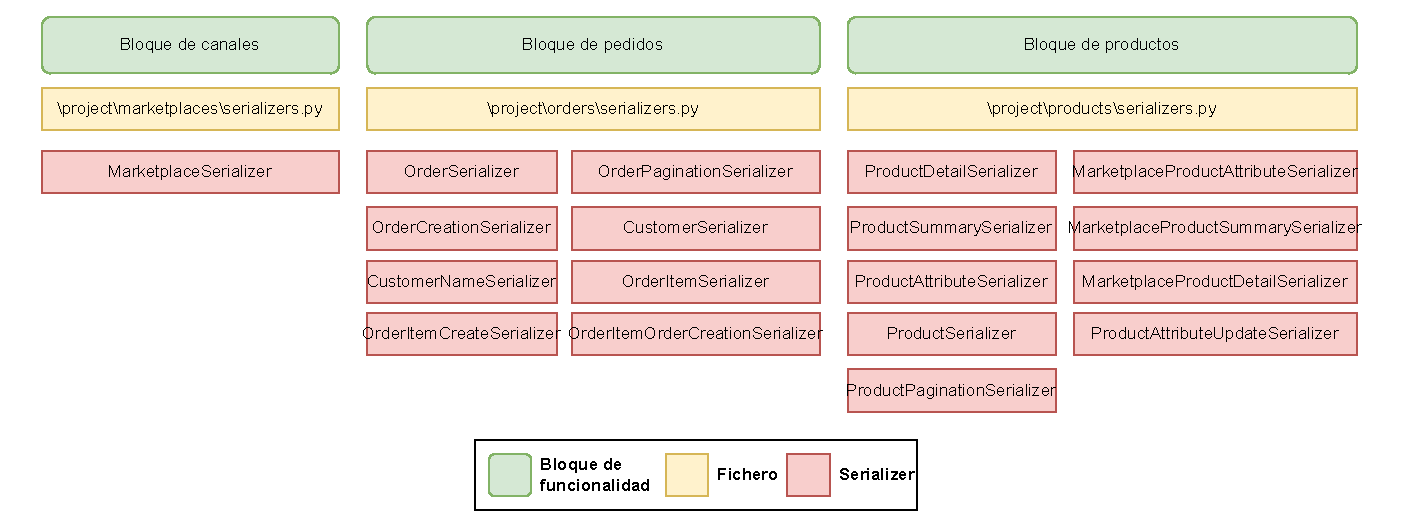
\includegraphics[width=0.95\textwidth]{figures/design_develop/estructura_serializers.pdf}
    \caption{Estructura de los \textit{serializers} del proyecto.}
    \label{dev:fig:estructura_serializers}
\end{figure}

En el apartado \ref{dev:subsec:definicion_vistas_urls} se explicará cómo se emplean estos \textit{serializers} dentro de las vistas y cómo se enlazan con las URLs correspondientes. Finalmente, en la sección \ref{dev:sec:desarrollo_frontend} se mostrará la aplicación práctica de cada \textit{serializer} en las distintas páginas del \textit{frontend}.

\subsection{Definición de las vistas y URLs}
\label{dev:subsec:definicion_vistas_urls}

Para finalizar el desarrollo del \textit{backend}, se deben definir las vistas y las URLs que llaman a dichas vistas. Las vistas son el componente encargado de gestionar las peticiones y respuestas de manera que cuando se acceda a una URL concreta, se ejecute la lógica necesaria para procesar la petición y devolver la respuesta adecuada. En el caso de una API REST, las vistas se encargan de recibir las peticiones HTTP, procesar los datos y devolver una respuesta en formato JSON.

En Django, las vistas se definen en el archivo \texttt{views.py} de cada aplicación, siguiendo una estructura coherente con la de los modelos y los \textit{serializers}. En el contexto de Django REST Framework, existen diversas formas de definir vistas, pero una de las más habituales consiste en utilizar vistas basadas en modelos junto con los denominados \textit{ViewSets}.

Estas vistas, al estar construidas sobre los modelos, permiten interactuar directamente con ellos, de forma análoga a como lo hacen los \textit{serializers}. El uso de \textit{ViewSets} facilita la definición de operaciones CRUD (Crear, Leer, Actualizar y Eliminar), ya que Django REST Framework proporciona métodos predefinidos para cada una de estas acciones. Gracias a esto, no es necesario implementar manualmente cada uno de los métodos básicos de la API que comparten todos los modelos. Dichos métodos que se implementan de forma automática son prácticamente equivalentes a los métodos del protocolo HTTP, descritos en la sección \ref{mt:subsec:api}, y son los siguientes:

\begin{itemize}
    \item \texttt{list}: Permite obtener una lista de todos los registros del modelo. Hace uso del método GET sin parámetros en la URL.
    \item \texttt{retrieve}: Permite obtener un registro concreto del modelo. Hace uso del método GET con un parámetro en la URL que indica el identificador del registro.
    \item \texttt{create}: Permite crear un nuevo registro del modelo. Hace uso del método POST con los datos del nuevo registro en el cuerpo de la petición.
    \item \texttt{update}: Permite actualizar un registro concreto del modelo. Hace uso del método PUT con el identificador del registro en la URL y los datos actualizados en el cuerpo de la petición.
    \item \texttt{partial\_update}: Permite actualizar parcialmente un registro concreto del modelo. Hace uso del método PATCH con el identificador del registro en la URL y los datos actualizados en el cuerpo de la petición.
    \item \texttt{destroy}: Permite eliminar un registro concreto del modelo. Hace uso del método DELETE con el identificador del registro en la URL.
\end{itemize}

No obstante, cuando se requiere una lógica más específica o se necesita implementar funcionalidades que no se cubren con los métodos estándar, es posible definir operaciones personalizadas dentro del propio \textit{ViewSet}.

\begin{center}
    \begin{minipage}{0.8\textwidth}
        \lstinputlisting[language=Python, caption={Definición del \textit{ViewSet} para el modelo \texttt{Customer}.}, label={lst:viewset}]{listings/viewset.py}
    \end{minipage}
\end{center}

En el fragmento de código \ref{lst:viewset} se puede observar un ejemplo de cómo se ha definido un \textit{ViewSet} para el modelo \texttt{Customer}. Este \textit{ViewSet} hereda de \texttt{viewsets.ModelViewSet}, lo que le otorga automáticamente los seis métodos mencionados anteriormente. Además de estos métodos, se ha añadido un método personalizado llamado \texttt{search} que a partir de un \textit{queryparam} permite buscar clientes por su dirección de correo electrónico. Por último, se ha definido un \textit{serializer\_class} que indica qué \textit{serializer} se debe utilizar para serializar los datos del modelo. En este caso, se ha utilizado el \textit{serializer} \texttt{CustomerSerializer}, que es el encargado de convertir los objetos del modelo \texttt{Customer} en formato JSON y viceversa. De esta manera, a esta vista se le pueden hacer las siguientes peticiones a través de las URLs:

\begin{itemize}
    \item \texttt{GET /customers/}: Devuelve una lista de todos los clientes.
    \item \texttt{GET /customers/\{id\}/}: Devuelve un cliente concreto por su identificador.
    \item \texttt{POST /customers/}: Crea un nuevo cliente.En el cuerpo de la petición se deben enviar los datos del nuevo cliente en formato JSON.
    \item \texttt{PUT /customers/\{id\}/}: Actualiza un cliente concreto por su identificador. En el cuerpo de la petición se deben enviar los datos actualizados del cliente en formato JSON.
    \item \texttt{PATCH /customers/\{id\}/}: Actualiza parcialmente un cliente concreto por su identificador. En el cuerpo de la petición se deben enviar los datos actualizados del cliente en formato JSON.
    \item \texttt{DELETE /customers/\{id\}/}: Elimina un cliente concreto por su identificador.
    \item \texttt{GET /customers/?q=\{email\}}: Busca clientes por su dirección de correo electrónico.
\end{itemize}

A cada uno de estos métodos con su correspondiente URL se les denomina \textit{endpoint}, y son los puntos de acceso a la API. Cada \textit{endpoint} corresponde a una operación concreta que se puede realizar sobre el modelo, y cada uno de ellos tiene una URL única que permite acceder a él. De esta manera, se puede interactuar con la API de forma sencilla y estructurada.

Habiendo escogido el enfoque de utilizar \textit{ViewSets} y habiendo mostrado un ejemplo de como estos funcionan, se ha definido la metodología a seguir para estructurar las vistas del proyecto. En primer lugar, se ha optado por crear un \textit{ViewSet} por cada modelo relevante, lo que permite agrupar las operaciones relacionadas con cada modelo en un único lugar. Esto facilita la organización del código y mejora la legibilidad, ya que cada \textit{ViewSet} se encarga de gestionar las operaciones de un único modelo y, en caso de requerir nuevas funcionalidades, se pueden añadir directamente en el \textit{ViewSet} correspondiente sin afectar al resto del proyecto.

La figura \ref{dev:fig:estructura_views} muestra la estructura general de las vistas del proyecto. Cada vista implementa los seis métodos predeterminados que proporcionan los \textit{ViewSets} y, además, incorpora los métodos personalizados para dar respuesta a necesidades específicas de la aplicación. Cada módulo cuenta con su propio archivo \texttt{views.py}, donde se definen los \textit{ViewSets} correspondientes a los modelos que forman parte de dicha aplicación.

\begin{figure}
    \centering
    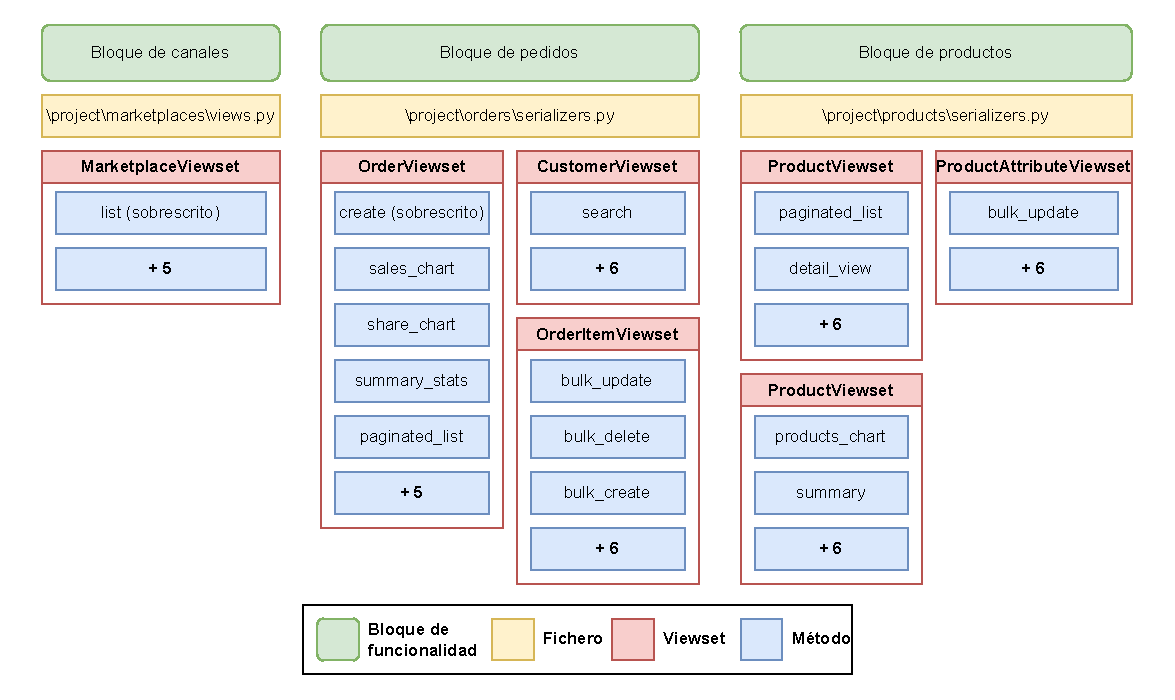
\includegraphics[width=0.95\textwidth]{figures/design_develop/estructura_views.pdf}
    \caption{Estructura de las vistas del proyecto.}
    \label{dev:fig:estructura_views}
\end{figure}

Finalmente, una vez definidos los \textit{ViewSets}, es necesario establecer las URLs que apuntan a cada uno de ellos. Esto se realiza en el fichero \texttt{urls.py} de cada aplicación, donde se definen las rutas que corresponden a cada \textit{ViewSet}. Análogamente, para enrutar cada una de las aplicaciones, se hace uso del fichero \texttt{urls.py} del directorio \texttt{project}, tal como se había ya descrito en la sección \ref{dev:subsec:estructura_proyecto}. De esta manera, se define una URL base para cada aplicación y, a partir de esta, se definen las URLs que apuntan a cada uno de los \textit{ViewSets}.

En la figura \ref{dev:fig:estructura_urls} se puede observar la estructura general de todas las URLs y los correspondientes métodos de los \textit{ViewSets} que se pueden solicitar al \textit{backend}. Cada URL corresponde a un \textit{endpoint} de la API, y cada uno de ellos tiene un método asociado que indica qué operación se puede realizar sobre el modelo. Por ejemplo, la URL \texttt{orders/customers/\{id\}/} corresponde al método \texttt{retrieve} del \textit{ViewSet} de \texttt{Customer} de la aplicación \texttt{orders}, lo que permite obtener un cliente concreto por su identificador.

\begin{figure}
    \centering
    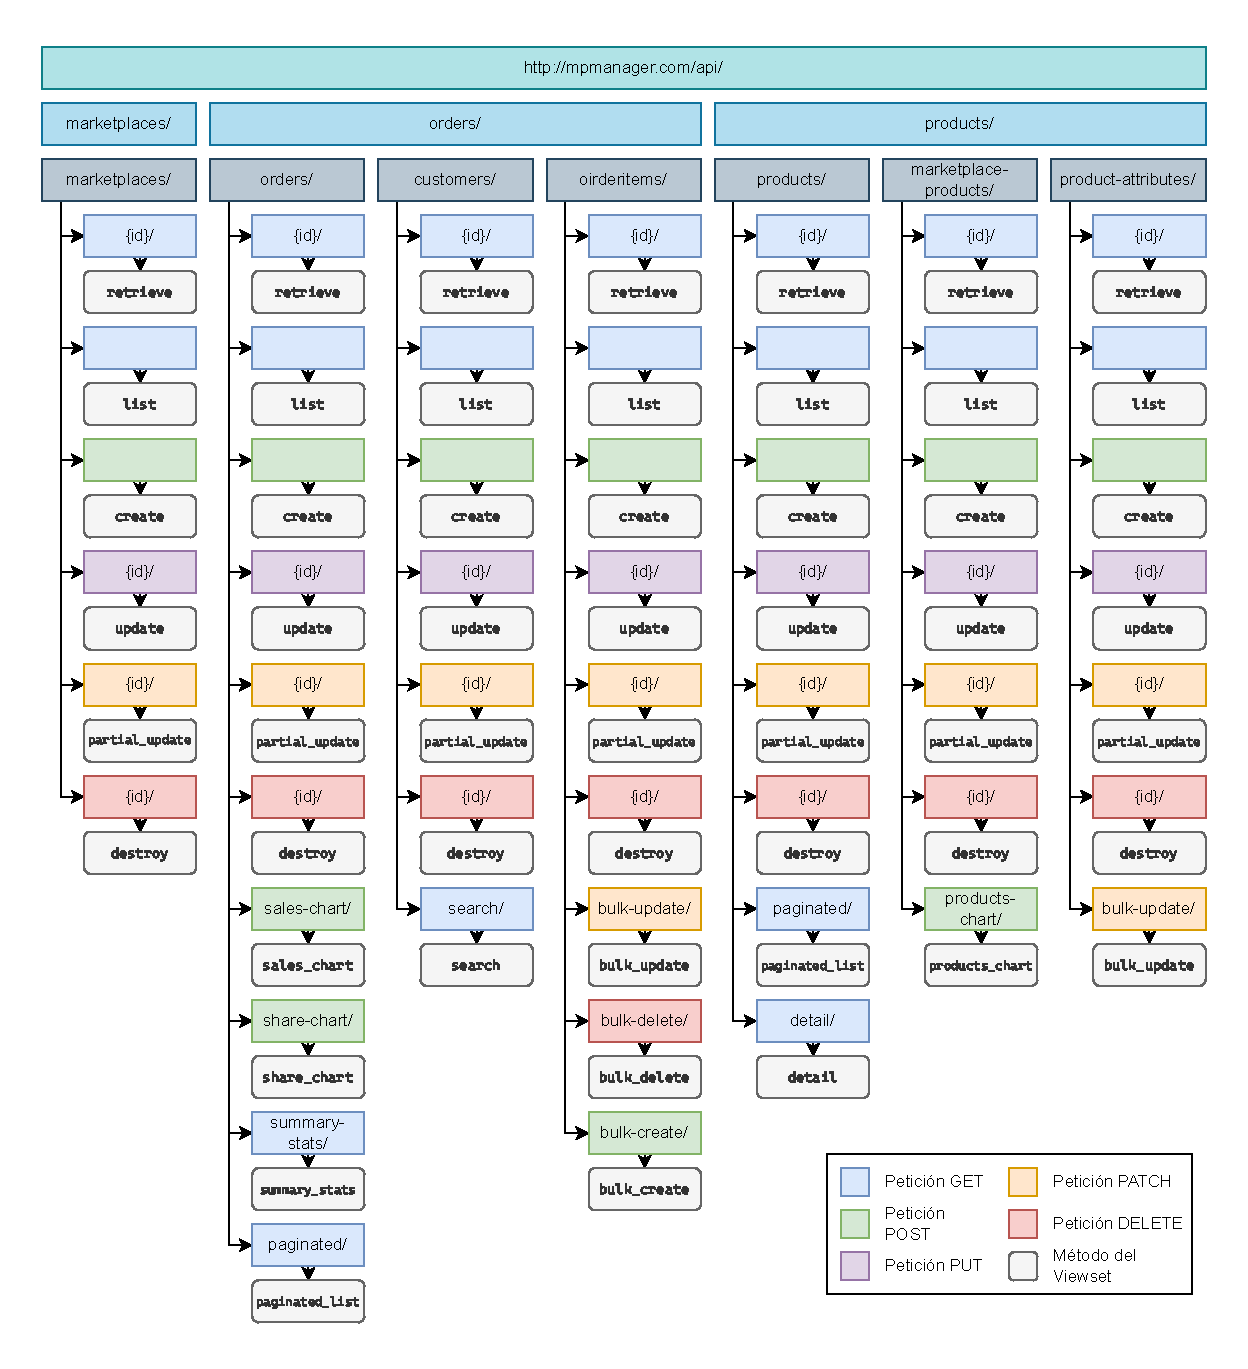
\includegraphics[width=0.95\textwidth]{figures/design_develop/estructura_urls.pdf}
    \caption{Enrutamiento de todas las URLs del \textit{backend} con sus correspondientes métodos de los \textit{ViewSets}.}
    \label{dev:fig:estructura_urls}
\end{figure}

Llegar a esta estructura de URLs ha sido un proceso iterativo, pues se ha tenido que cambiar varias veces a medida que la aplicación ha ido evolucionando y el \textit{frontend} ha ido requiriendo nuevos \textit{endpoints}. Estructurar el enrutamiento de tal cantidad de \textit{endpoints} es complejo y supone un reto si se quiere hacer correctamente de manera que en un futuro se puedan añadir funcionalidades si alterar mucho lo ya existente. Sin embargo, se ha tratado de mantener una estructura coherente y lógica, de manera que solamente leyendo las URLs se pueda entender qué operaciones se pueden realizar sobre cada modelo y cómo se pueden acceder a ellas.

\subsection{Implementaciones relevantes}
\label{dev:subsec:implementaciones_relevantes}

Para cerrar la sección de desarrollo del \textit{backend}, es importante destacar algunas implementaciones relevantes que han requerido una atención especial por su complejidad o impacto funcional. Entre ellas, se encuentra la incorporación de un sistema de paginación para optimizar la entrega de datos en la API, así como la incorporación de distintos métodos para la actualización, creación y eliminación de entidades de manera masiva.

\subsubsection{Paginación de \textit{endpoints}}
\label{dev:subsubsec:paginacion_endpoints}

Cuando se manejan grandes volúmenes de datos, la paginación se convierte en una herramienta fundamental para garantizar una experiencia de usuario fluida y eficiente. Como se ha mencionado anteriormente, a mayor cantidad de datos transmitidos, mayor será el tamaño de la respuesta y, en consecuencia, más lenta será la carga de la página. Por este motivo, en aquellas vistas donde se espera un listado extenso de elementos, resulta imprescindible implementar un sistema de paginación que permita dividir los resultados en páginas más pequeñas y manejables.

Un \textit{endpoint} con paginación permite que, mediante el uso de \textit{query parameters}, el cliente especifique tanto el número de resultados por página como la página concreta que desea consultar. En la mayoría de los casos, al usuario no le interesa obtener todos los resultados de forma simultánea, sino acceder progresivamente a los datos en función de su necesidad concreta.

Adicionalmente a la paginación, en muchos casos también es útil poder filtrar los resultados según ciertos criterios o realizar búsquedas específicas. Por ejemplo, en un listado de productos, el usuario podría querer ver solo aquellos que cumplen con ciertas características o que pertenecen a una categoría específica. Para ello, se pueden añadir \textit{query parameters} adicionales que permitan filtrar los resultados según los criterios deseados.

Volviendo a la figura \ref{dev:fig:estructura_urls}, se puede observar que existen dos \textit{endpoints} que incorporan paginación: uno para listar los pedidos y otro para listar los productos. Estos dos \textit{endpoints} van a ser esenciales en sus correspondientes páginas del \textit{frontend}, de manera que hacer que sus respuestas sean lo más eficientes posible es crucial para garantizar una buena experiencia de usuario.

Para detallar de manera más práctica la implementación de la paginación, se va a tomar como ejemplo el \textit{endpoint} de los pedidos. En este caso, la URL es la siguiente:

\begin{center}
    \texttt{GET /orders/paginated/?page=\{n\}\&limit=\{m\}\&marketplace\_ids=\{ids\}\&search=\{query\}}
\end{center}

En esta URL, se pueden observar los siguientes \textit{query parameters}:
\begin{itemize}
    \item \texttt{page}: Indica el número de página que se quiere consultar. Por defecto, si no se especifica, se toma el valor 1.
    \item \texttt{limit}: Indica el número de resultados por página. Por defecto, si no se especifica, se toma el valor 10.
    \item \texttt{marketplace\_ids}: Permite filtrar los pedidos por los identificadores de los \textit{marketplaces} asociados. Si no se especifica, se obtienen todos los pedidos.
    \item \texttt{search}: Permite buscar pedidos por un término concreto. Si no se especifica, no se realiza ninguna búsqueda.
\end{itemize}

Realizando una petición a esta URL, se obtiene una respuesta en formato JSON que contiene los pedidos correspondientes a la página solicitada, así como información adicional sobre la paginación. Esta información incluye el número total de páginas, el número total de resultados y el número de resultados por página. De esta manera, el cliente puede saber cuántas páginas hay en total y cuántos resultados hay en cada página, lo que le permite navegar por los resultados de manera más eficiente.

\subsubsection{Actualización, creación y eliminación masiva}
\label{dev:subsubsec:actualizacion_creacion_eliminacion_masiva}

En muchas ocasiones, es necesario realizar operaciones masivas sobre los datos, como actualizar, crear o eliminar múltiples registros de una sola vez. Hacer tantas peticiones como registros a modificar puede resultar ineficiente y generar una carga innecesaria en el servidor, especialmente si se trata de un gran número de registros. Por este motivo, se ha implementado la posibilidad de realizar estas operaciones de forma masiva a través de un único \textit{endpoint} para determinados modelos, tal como se puede observar en la figura \ref{dev:fig:estructura_urls} bajo los métodos que incluyen la palabra \textit{bulk}.

En concreto, el principal modelo al que se ha aplicado esta funcionalidad es el de \texttt{OrderItem}, que representa los productos de un pedido. La necesidad de implementar operaciones masivas en este modelo se podrá observar en la debida sección del \textit{frontend}; sin embargo, es fácilmente comprensible que, al gestionar pedidos con múltiples productos, la posibilidad de actualizar, crear o eliminar varios productos de un pedido de forma simultánea resulta prácticamente indispensable.

En concreto, se han implementado tres operaciones masivas para el modelo \texttt{OrderItem}:

\begin{itemize}
    \item \texttt{bulk\_update}: Haciendo uso del método PATCH, permite actualizar múltiples productos de un pedido de forma simultánea. La petición debe incluir en el cuerpo un listado de productos con sus respectivos identificadores y los campos a actualizar.
    \item \texttt{bulk\_create}: Haciendo uso del método POST, permite crear múltiples productos de un pedido de forma simultánea. La petición debe incluir en el cuerpo un listado de productos con los datos necesarios para su creación.
    \item \texttt{bulk\_delete}: Haciendo uso del método DELETE, permite eliminar múltiples productos de un pedido de forma simultánea. La petición debe incluir en el cuerpo un listado de identificadores de los productos a eliminar.
\end{itemize}